%\documentclass[9pt,twocolumn,twoside]{osajnl}
%\journal{ol} % Choose journal (ao, ol, josaa, josab)
%\setboolean{shortarticle}{true} % true = letter, false = research article
%\documentclass[twocolumn]{article}
\documentclass[10pt,letterpaper]{article}
\usepackage{opex3}
\usepackage{color}

\usepackage[utf8x]{inputenc}
\usepackage[colorlinks=true,linkcolor=black,citecolor=black,pdfusetitle,pagebackref=false]{hyperref}
\usepackage[nonumberlist,nohypertypes={glossary}]{glossaries}
\usepackage{graphicx}
\usepackage{multicol}
\usepackage[font=small,labelfont=bf]{caption}
\usepackage{subcaption}
%\usepackage{authblk}
\usepackage{amsmath}
\usepackage{bm}
\usepackage[margin=1.5cm]{geometry}
%\usepackage{cite}
%\usepackage[usenames,dvipsnames,svgnames,table]{xcolor}
%\usepackage{bigints}
%\usepackage[normalem]{ulem}
%\usepackage{mathrsfs}



\newenvironment{Figure}
  {\par\medskip\noindent\minipage{\linewidth}}
  {\endminipage\par\medskip}

\bibliographystyle{unsrt}
\renewcommand\refname{References}

\newacronym{cdi}
    {CDI}{coherent diffractive imaging}

\newacronym{odt}
    {ODT}{optical dipole trap}

\newacronym{bec}
    {BEC}{Bose-Einstein condensate}

\newacronym{fort}
    {FORT}{far-off-resonance trap}

\newacronym{ta}
    {TA}{tapered amplifier}

\newacronym{caes}
    {CAES}{cold-atom electron source}

\newacronym{xfel}
    {XFEL}{x-ray free electron laser}

\newacronym{mot}
    {MOT}{magneto-optical trap}

\newacronym{ecdl}
    {ECDL}{external cavity diode laser}

\newacronym{aom}
    {AOM}{acousto-optical modulator}

\newacronym{slm}
    {SLM}{spatial light modulator}

\newacronym{mopa}
    {MOPA}{master-oscillator power amplifier}

\newacronym{na}
    {NA}{numerical aperture}

\newacronym{ar}
    {AR}{anti-reflection}

\newacronym{ccd}
    {CCD}{charge-coupled device}

\newacronym{cro}
    {CRO}{cathode ray oscilloscope}

\newacronym{pbs}
    {PBS}{polarising beam splitter}

\newacronym{bs}
    {BS}{beam splitter}

\newacronym{npbs}
    {NPBS}{non-polarising beam splitter}

\newacronym{tec}
    {TEC}{thermo-electric cooler}

\newacronym{cw}
    {CW}{continuous wave}

\newacronym{mcp}
    {MCP}{microchannel plate}

\newacronym{fwhm}
    {FWHM}{full-width half maximum}

\newacronym{pdh}
    {PDH}{Pound-Drever-Hall}
    
\newacronym{ps}
    {PS}{polarisation spectroscopy}
    
\newacronym{obe}
    {OBE}{optical Bloch equation}
    
\newacronym{davll}
    {DAVLL}{dichroic atomic vapour laser lock}

\newacronym{mts}
    {MTS}{modulation transfer spectroscopy}

\newacronym{snr}
    {SNR}{signal-to-noise ratio}

\newacronym{lsd}
    {LSP}{linear spectral density}


\makeglossaries

\begin{document}

\title{kHz linewidth lasers using polarisation spectroscopy}
\author{J. S. J. Torrance, B. M. Sparkes, and R. E. Scholten}
\address{School of Physics, The University of Melbourne, Melbourne, Victoria 3010 Australia}
%\dates{Compiled \today}

%\ociscodes{(140.3490) Lasers, distributed feedback; (060.2420) Fibers, polarization-maintaining;(060.3735) Fiber Bragg gratings.}


\begin{abstract}
Polarisation spectroscopy is a laser frequency stabilisation technique that probes the birefringence induced in an atomic medium by a circularly polarised pump laser beam. Due to polarisation spectroscopy being a refractive index based technique it is not limited by the lifetime of atomic states, unlike similar techniques such as saturated absorption spectroscopy. Polarisation spectroscopy has been shown to offer high bandwidth locking to an atomic reference, and linewidth narrowing, without requiring radio-frequency electronics. We investigate the noise-limited bandwidth of polarisation spectroscopy frequency discrimination and demonstrate sub-kHz laser linewidths with conventional \gls*{ecdl} using two similar setups and a heterodyne measurement.
\end{abstract}

%\setboolean{displaycopyright}{true}

%\maketitle
%\thispagestyle{fancy}
%\ifthenelse{\boolean{shortarticle}}{\abscontent}{}
%\begin{multicols}{2}

%\section{Intro}
%Laser frequency stabilisation to atomic references is essential to numerous applications including the cooling and trapping of atoms\cite{uetake_high_2008, ye_stable_2010, akamatsu_narrow_2012} and high resolution spectroscopy\cite{rafac_sub-dekahertz_2000}. In addition to stabilising the frequency, narrowing the specral linewidth of lasers is important to applications such as atomic clocks\cite{ludlow_sr_2008} and metrology\cite{metcalf_laser_1999, ye_quantum_2008, demtroder_laser_2003}.
%
%There are a number of desirable traits in laser frequency stabilisation schemes such as being able to stabilise to an atomic reference, being free of frequency modulation, having high bandwidth in order to achieve low spectral linewidths, simplicity of implementation and low cost.
%
%Current techniques for linewidth stabilisation range from saturated absorption spectroscopy, which can achieve diode laser linewidths in the region of 150\,kHz\cite{cuneo_optically_1994}, to elaborate experiments involving extremely high finesse cavities that are able to achieve sub-Hertz linewidths with diode lasers using the \gls*{pdh} technique\cite{ludlow_compact_2007}.
%
%The ability to stabilise a laser's frequency to an atomic reference, rather than to an abitrary frequency, is frequently essential to experiments. Techniques such as saturated absorption spectroscopy\cite{maguire_theoretical_2006, haroche_theory_1972, preston_doppler-free_1996}, \gls*{davll}\cite{corwin_frequency-stabilized_1998,millett-sikking_davll_2007}, \gls*{mts}\cite{shirley_modulation_1982, mccarron_modulation_2008,xiang-hui_ultra-stable_2009} and Sagnac interferometry\cite{robins_Interferometric_2002,jundt_non-linear_2003} lock to atomic references whereas optical cavity techniques such as \gls*{pdh}\cite{drever_laser_1983} do not. \Gls*{ps} is another technique that stabilises a laser's frequency to an atomic transition although \gls*{ps} performs significantly better on closed transitions than open ones\cite{pearman_polarization_2002}.
%
%Frequency modulation of the laser is required for some locking techniques but it can interfere with experimental applications so it is often desirable to avoid direct modulation of the laser's frequency using techniques such as \gls*{ps} or \gls*{davll} or by modulating only one beam from the laser using an \gls*{aom} or similar. This can be achieved with techniques that do not require modulation or by modulation of only the beam used in the locking setup using \glspl*{aom} or similar. \Gls*{ps} is a technique that requires no modulation.
%
%\Gls*{ps} schemes involve only slightly more components than saturated absorption spectroscopy setups and are significantly simpler that those required for techniques such as \gls*{pdh} or \gls*{mts} meaning that setup time, expertise and cost are competitive with the simplest locking techniques.
%
%It has been shown previously that \gls*{ps} can be used to reduce the linewidth of a distributed feedback diode from 2\,MHz to 20\,kHz\cite{torii_laser-phase_2012} and of diode lasers to 65\,kHz\cite{yoshikawa_frequency_2003}. Our \gls*{ps} locking system utilises high bandwidth feedback to the laser diode to achieve linewidths of order 1\,kHz.
%
%Some locking techniques are limited by the evolution of the atomic states which evolve slower than the lifetime of the excited state (26.2\,ns for Rb85). Unlike these techniques \gls*{ps} is not limited by the rates at which the atomic populations evolve. At high frequency \Gls*{ps} depends on interactions with the refractive index of the atomic medium and is thus technically and noise limited.
%
%\section{Pol Spec Theory}
%
%%\begin{Figure}
%%    \centering
%%    \captionsetup{type=figure}
%%    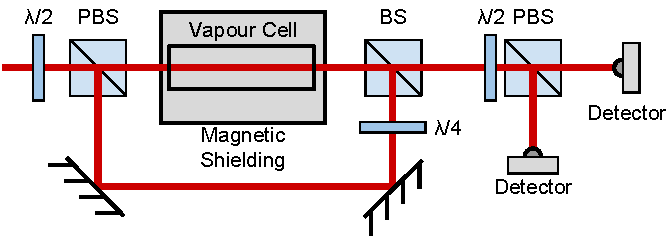
\includegraphics[width=\linewidth]{Figs/PolSpec.pdf}
%%    \captionof{figure}{A schematic of polarisation spectroscopy with a balanced polarimeter. The power balance between the probe and pump beam is controlled with the leftmost $\lambda/2$ waveplate and \glsfirst*{pbs}. The $\lambda/4$ waveplate is used to make the pump circularly polarised and the non-polarising \gls*{bs} is used to make the beams colinear and counter-propagate them through the atomic sample without altering the polarisation of the circular pump or linear probe. The final $\lambda/2$ waveplate and \gls*{pbs} form the balanced polarimeter which monitors the polarisation rotation of the probe.}
%%    \label{polspec_schematic}
%%\end{Figure}
%
%A schematic diagram for \gls*{ps}\cite{wieman_doppler-free_1976, demtroder_laser_2014} is shown in figure \ref{polspec_schematic}. A circularly polarised pump beam from a monochromatic tunable laser is used to induce frequency dependent, circular birefringence in an atomic gas sample by optically pumping the atoms. A linearly polarised beam from the same laser is used to probe the birefringence since the probe's polarisation is rotated by the birefringence. To prevent Faraday rotation the atomic sample is shielded from external magnetic fields. A measurement of the probe's polarisation rotation gives a frequency dependent error signal which can be used for laser locking to atomic transitions.
%
%The polarisation rotation of the probe is monitored using a balanced polarimeter consisting of a half-wave plate, \gls*{pbs} and two detectors. The difference between the signals from the two detectors provides a background-free signal ideal for locking\cite{pearman_polarization_2002}.
%
%Neglecting the birefringence of the windows of the atomic cell for simplicity, the error signal for \gls*{ps} is given by the difference in intensity at the two detectors,\cite{pearman_polarization_2002}
%\begin{align}
%I_{PS} = I_x-I_y = -I_0 \cos(2\phi+2\Phi)\label{I_PS}
%\end{align}
%where $I_x$ ($I_y$) is the horizontal (vertical) linearly polarised component of the probe after the sample, $I_0$ is the intensity of the probe in the absence of a pump beam, $\phi$ is the angle of polarisation of the probe in the absence of a pump beam and $\Phi$ is the additional rotation due to the birefringence induced by the pump. The largest \gls*{ps} spectrum is produced when $\phi=\pi/4$ and since $\Phi$ is small equation \ref{I_PS} can be approximated to
%\begin{align}
%I_{PS} \approx I_0 2\Phi
%\end{align}
%
%If we define the difference in refractive indices for the $\sigma^\pm$ components of the probe, $n_\pm$, as $\Delta n = n_+ - n_-$ then we can write\cite{hecht_optics_1987}
%\begin{align}
%\Phi = \frac{\pi L \Delta n}{\lambda}
%\end{align}
%where $L$ is the length of the atomic sample and $\lambda$ is the wavelength of the laser light.
%
%The spectral profile of the difference in absorption coeffients for the medium in the vicinity of a resonance is a Lorentizian with \gls*{fwhm} $\Gamma$\cite{demtroder_laser_2003}:
%\begin{align}
%\Delta \alpha = \frac{\Delta\alpha_0}{1+4\left(\frac{\delta}{\Gamma}\right)^2}.
%\end{align}
%Here, $\delta=\omega_L-\omega_A$ is the detuning of the laser from the resonance where $\omega_L$ is the angular frequency of the laser and $\omega_A$ the angular frequency of the atomic resonance. $\Delta\alpha_0$ is the difference in absorption cooefficients for the $\sigma^\pm$ circular polarisation components at $\delta=0$ and $\Gamma$ is the lifetime of the excited state of the resonance transition.
%
%The refractive index and absorption coefficient of the medium can then be related through the Kramers-Kronig dispersion relation\cite{demtroder_laser_2003} to give
%\begin{align}
%\Delta n = \Delta\alpha_0 \frac{2c}{\omega_0 \Gamma}\frac{\delta}{1+4\left(\frac{\delta}{\Gamma}\right)^2}\label{result}
%\end{align}
%
%The only term left to be determined in equation \ref{result} is $\Delta\alpha_0$, the maximum difference in absorption coefficients, which occurs at the line centre where $\delta=0$. For a weak probe beam $\Delta\alpha_0$ depends only on the effects of the pump.
%
%The steady state behaviour of $\Delta n$ has been dealt with by Hughes\cite{hughes_polarization_2009}{\color{red} (Why do we care. Explain.)}.
%
%{\color{red}We need more of a description of how $\Delta\alpha_0$ is calculated. Hopefully linking in the populations/density matrix.
%
%according to Hughes in that book...}
%
%\begin{align}
%\Delta\alpha = \int \mathscr{A}(t)\mathscr{H}(t)dt
%\end{align}
%Here the time dependent anisotropy of the medium is given by
%\begin{align}
%\mathscr{A}(t)=\sum_{m_F} \alpha_{(F,m_F\rightarrow F',m_{F+1})}(P_{F,m_F}-P'_{F',m_{F+1}})\\
%-\alpha_{(F,m_F\rightarrow F',m_{F-1})}(P_{F,m_F}-P'_{F',m_{F-1}})
%\end{align}
%
%But where do I get $\alpha$ from??
%
%{\color{red}Hughes thing ends here}
%
%The atomic substate populations and coherences that define the density matrix $\rho$ {\color{red}[cite someone on density matrices]} evolve at rates limited by the spontaneous decay time. Laser frequency noise can extend to much higher frequencies, and thus the polarisation spectroscopy signal of equation {\color{red} 5?} can provide feedback bandwidth not limited by the usual absorption (spontaneous) decay bandwidth of $\Gamma/2$ (3\,MHz in the case of Rb). Equivalently, the useful frequency range of the \gls*{ps} error signal is many times broader than can be obtained from absorption-based atomic references, allowing stabilisation to frequencies far from resonance. {\color{red} reference to ps/satabs spectra.}
%
%An example of a \gls*{ps} error spectrum for rubidium 85 5$^\text{2}$S$_\text{1/2}$ to 5$^\text{2}$P$_\text{3/2}$ transition is given in figure \ref{polspec_spectrum}.
%
%%\begin{Figure}
%%    \centering
%%    \captionsetup{type=figure}
%%    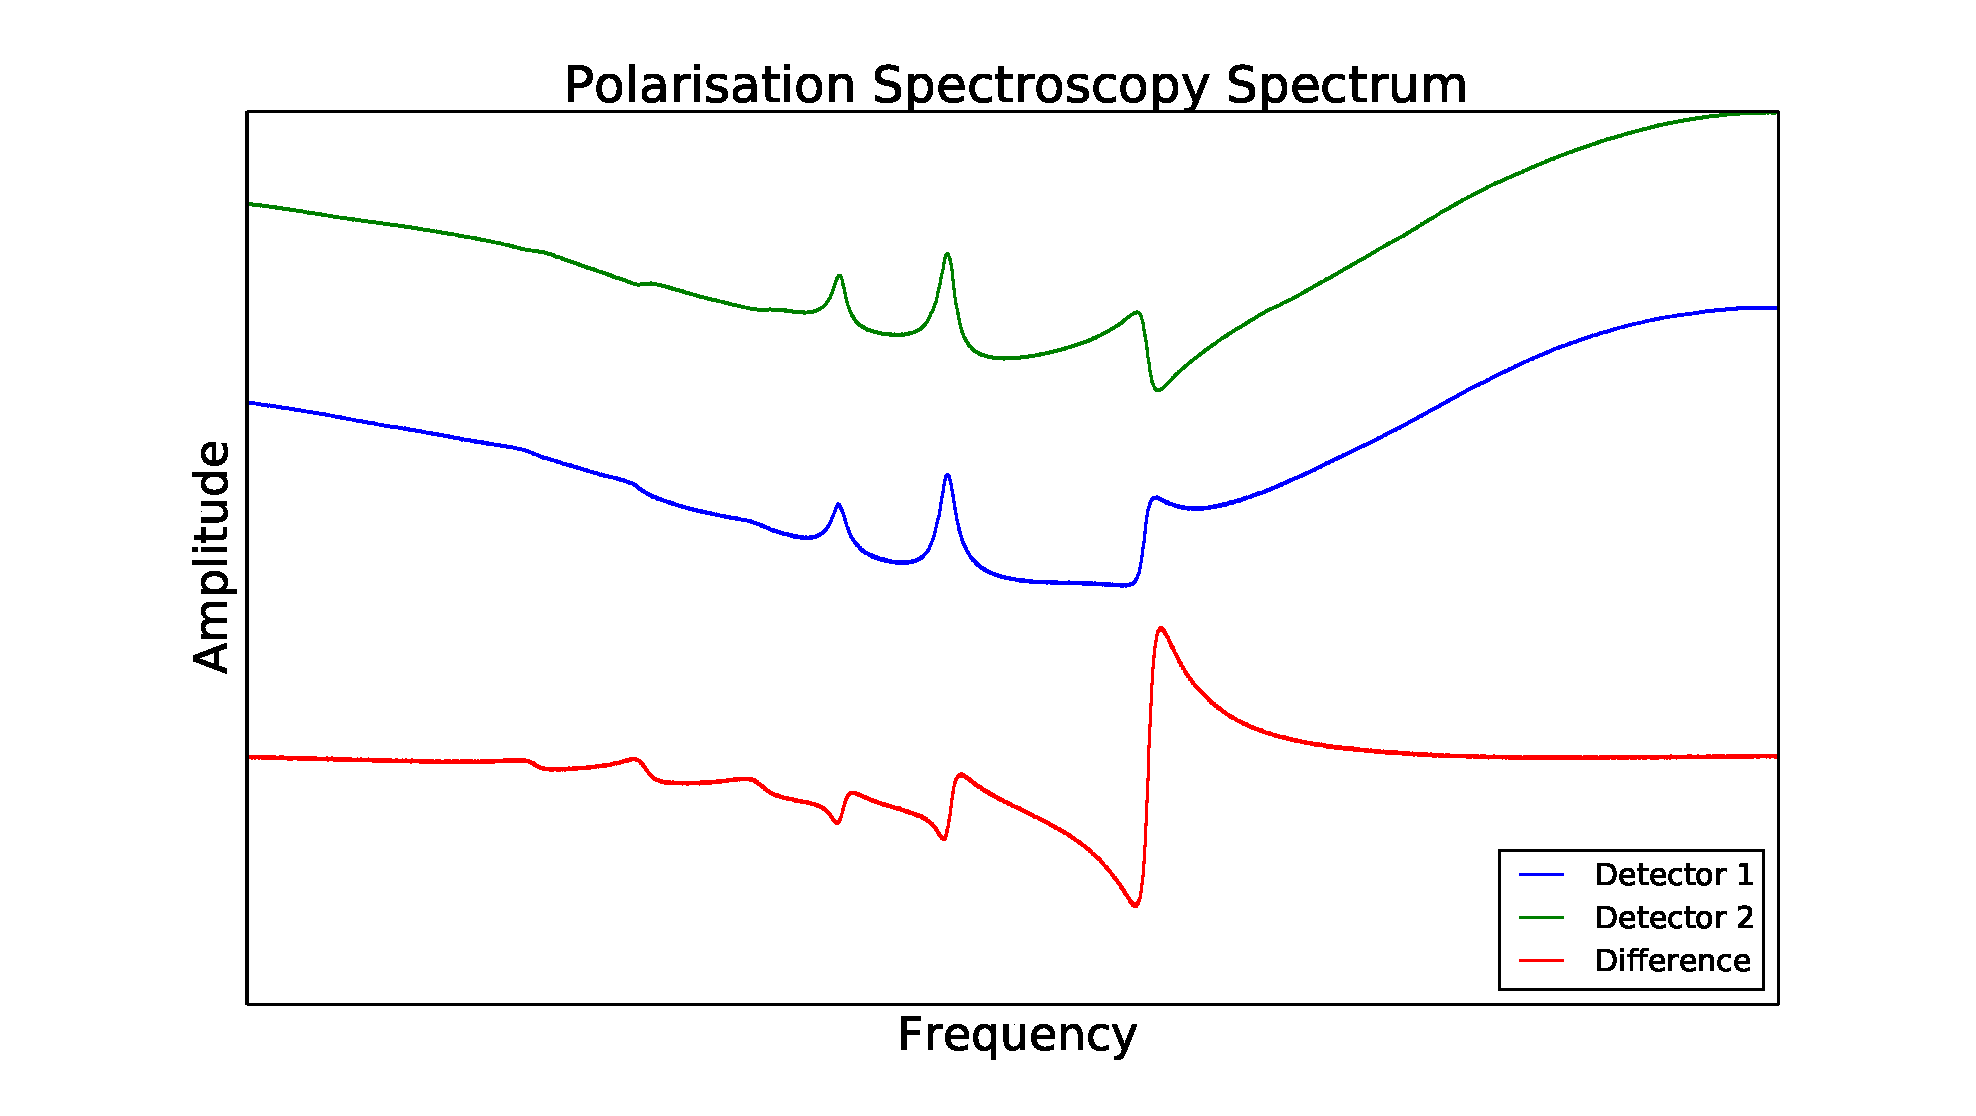
\includegraphics[width=\linewidth]{Figs/spectrum.pdf}
%%    \captionof{figure}{An example of the polarisation spectrum of the Rb85 5$^\text{2}$S$_\text{1/2}$ to 5$^\text{2}$P$_\text{3/2}$ transition. This is a stand in image. One showing pol spec vs sat abs would probably be more useful. Label the various transitions too.}
%%    \label{polspec_spectrum}
%%\end{Figure}
%
%{\color{red}Bandwidth theory? Possibly have to noise then to linewidth.\cite{di_domenico_simple_2010}}
%
%\section{Experiment}
%
%Two separate \glspl*{ecdl} were individually locked using \gls*{ps} and high bandwidth feedback. The lasers are controlled with commercial laser controllers\cite{mogbox} for temperature control, current supply and piezo control. A heterodyne measurement was then made to determine the lasers' spectral linewidths. 780\,nm laser diodes were used to target the rubidium 85 D2 F=3 to F$'$=4 transition.
%
%The two lasers used had modulation bandwidths {\color{red}(be more specific - fast feedback modulation bandwidths?)} of 100\,MHz\cite{dl_pro} and {\color{red}???}\,MHz\cite{mog_ecd003}. Both laser beams were split by a \gls*{pbs} and the subsquent beams were then fibre coupled into polarisation maintaining fibres. The output of the fibres led to the \gls*{ps} locking and the heterodyne measurement.
%
%The polarisations of the locking beams are stabilised with Glan-Thompson prisms before entering the \gls*{ps} setup shown in figure \ref{polspec_schematic}. Telescopes are used to increase the width of the locking beams, allowing them to interact with more atoms thus increasing $|\Delta\alpha_0|$\cite{demtroder_laser_2003} and improving the \gls*{snr}.
%
%The \gls*{ps} detectors were 100\,MHz bandwidth photodiodes\cite{tl_det} the outputs of which were connected to 14\,MHz bandwidth servo controllers\cite{nf_servo}. The servo controllers handled the subtraction of the balanced polarimetres detector signals to produce the error signal as well as locking parameters such as gain curves. The output of the servo controllers was connected to the fast modulation inputs of the lasers.
%
%The heterodyne measurements were made by first frequency shifting one of the laser beams with an \gls*{aom} and then combining the two beams to be colinear and coincident onto a 1\,GHz high bandwidth detector\cite{nf_det}. The output of this detector is given to the 40\,GHz bandwidth spectrum analyser\cite{rs_sa} and the heterodyne signal can be measured centred around the the \gls*{aom} frequency if both lasers are locked to the same atomic transition.

\section{Results}

\subsection{Frequency Noise Measurements}
%{\color{red} Noise measurements with eagle eye and uber cavity?}
%{\color{red} Changed the focus from bandwidth to noise. Write with this in mind and liberal citations of \cite{negnevitsky_wideband_2013}.}

\begin{Figure}
    \centering
    \captionsetup{type=figure}
    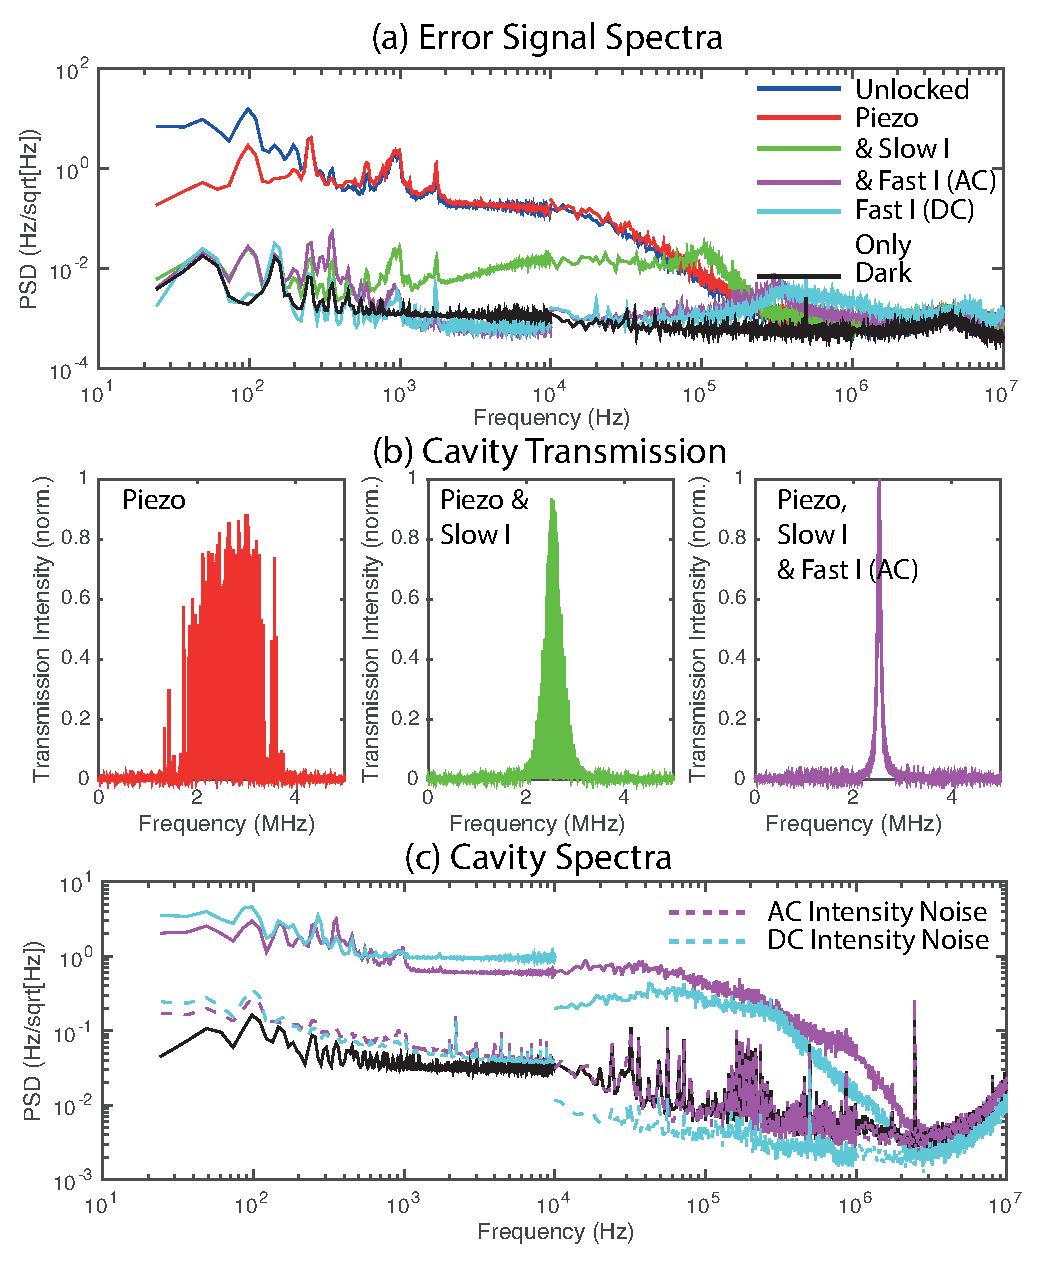
\includegraphics[width=\linewidth]{Figs/150904_SpectralDensityPlotsV102.eps}
    \caption{Frequency Noise Measurements. (a) Linear spectral density (LSD) measurements of polarisation spectroscopy error signal frequency noise for a range of laser locking regimes: Piezo = piezo-only locking; Slow I = slow current feedback (40~kHz bandwidth); Fast I = fast current feedback (maximum 14~MHz bandwidth) fed straight to the diode either AC-coupled in combination with piezo and slow I feedback, or DC-coupled feedback only. (b) Cavity transmission intensity as a function of AOM frequency scanning around resonance for different locks. Cavity HWHM linewidth is 70~kHz, scan time was 10~ms. (c) LSD measurements of transmitted cavity signal at half peak height for high-bandwidth locks. Also shown are the intensity noise of the laser, measured by removing the cavity and measuring frequency fluctuations with an intensity equal to half the peak transmission intensity. For (a) and (c) noise below $10^4$~Hz was measured using a computer sound card with a resolution bandwidth (RBW) of 12.2~Hz, noise between $10^4$-$10^6$~Hz was measured with an spectrum analyser with a RBW of 30~Hz, and measurements above $10^6$~Hz were measured with a spectrum analyser with a RBW of 300~Hz.}
    \label{noise_measurement}
\end{Figure}

We investigated the efficacy of the polarisation spectroscopy locking set-up by analysing the error signal created. The frequency noise linear spectrum density (square-root of power spectral density) was determined with a computer sound card (low frequency) and RF spectrum analyser (medium and high frequency). The spectrum analyser was calibrated using the slope of the error signal and the known input impedance, while the sound card data was \textit{matched} to the spectrum analyser data. Figure~\ref{noise_measurement}(a) shows the noise spectra for a number of different cases, with ``AC'' and ``DC'' referring to whether the laser head board was AC- or DC-coupled respectively \textit{(AC cut-off=?)}. For the AC case, the piezo and low-bandwidth current feedback were also implemented, this was not the case for the DC locking, where all feedback was supplied through the fast current modulation input. Unsurprisingly, as the bandwidth of the locking increased, so did the reduction in noise, with the bandwidth of the piezo-only feedback being of order 200~Hz, slow current feedback being 70~kHz, and fast locking being 200~kHz. \textit{Something about Bode bumps?}\\

The measurement of noise on the error signal for the fast current feedback is limited by the dark noise, measured by blocking the detectors, below approximately 30~kHz. This is due, in part, \textit{to the suppression of noise within the feedback loop}. A more sensitive and precise measure of the frequency spectra requires a frequency discriminator. In this case we chose to use an ultra-stable cavity with a half-width-at-half-maximum (HWHM) linewidth of 70~kHz. The narrow linewidth of the cavity allowed us to measure noise up to 10~MHz, limited by the bandwidth of the detector. Figure~\ref{noise_measurement}(b) shows cavity transmission signals as the laser frequency is scanned with an AOM, with a sweep time of 10~ms. The resulting traces provide a clear illustration of the effect of increased locking bandwidth: with piezo locking only the peak appears broad as the laser jitters around the resonant frequency on the 10~ms timescale, as slow current feedback is applied the peak becomes narrower and taller, and finally we see the effect of high-bandwidth modulation with a peak that has a HWHM limited by the cavity finesse, indicating a laser linewidth much smaller than 70~kHz.\\

By choosing a static AOM frequency such that the transmitted laser intensity is half the peak intensity, and therefore the transmission-frequency response is approximately linear, we can analyse the frequency noise of the laser through the cavity transmission signal. This is shown in Fig.~\ref{noise_measurement}(c) for both the fast AC and DC locking, both now well above the dark noise. The other locks shown in Fig.~\ref{noise_measurement}(a) cannot be evaluated using this method, as they were too noisy to stay within the linear frequency response range of the cavity. The AC and DC locks are both flat at low frequencies, reducing above 50~kHz. The peaks in the dark noise between $10^4$ and $10^6$~Hz are due to electronic pick-up by the detector. The drawback of this method is that laser intensity noise is mapped into frequency noise. The laser intensity noise spectrum, measured at the same power as the locked transmission signal, is also shown in Fig.~\ref{noise_measurement}(c). The intensity noise is well below the cavity transmission noise and we can therefore assume that the measured spectrum is dominated by the frequency fluctuations of the laser.\\

We can extract a linewidth for the laser from the cavity data using two methods: first we can use the known bandwidth of the cavity to map the locked transmission signal to a \textit{Gaussian/Lorentzian peak} and measure its linewidth \textit{(Josh, is this correct?)}. For our system this gives a linewidth of ?? \textit{approximately 5~kHz}. This method is sensitive to the laser intensity noise. To illustrate this, calculating a laser linewidth from the intensity noise gives a linewidth of ??, indicating that the real laser linewidth \textit{is well below this value}. To extract an exact linewidth with this method, a cavity with a higher finesse would be required. The second method involves integrating the power spectral density to determine the rms linewidth \textit{[cite negnevitsky2013]}. Performing this for the AC lock gives an rms linewidth of 350~Hz. Assuming the linewidth has a Gaussian shape gives a FWHM linewidth of approximately 850~Hz, much lower than that calculated using the above method. The results from these methods are summarised in Table~\ref{linewidth_table}.\\

\begin{table}[h!]
\centering
\begin{tabular}{|c|c|}
\hline \hline
Method & Linewidth (kHz) \\ \hline
(i) Map Gaussian (intensity) & 5 ?? \\
(ii) Map Gaussian (frequency) & 5 ?? \\
(iii) PSD Integral & 0.85 \\
(iv) Heterodyne & 1 ?? \\
\hline \hline
\end{tabular}
\caption{Linewidth calculation methods and results obtained. The mapping the transmission signal through a cavity with a HWHM of 70~kHz to a Gaussian signal [(i) and (ii)] is limited by the laser intensity noise. The results from integrating the power-spectral density signal (Fig.~\ref{noise_measurement}) and the Heterodyne beat-note (Fig.~\ref{beatnote}) both give a value for the linewidth of less than 1~kHz.}
\label{linewidth_table}
\end{table}

%\begin{table}[h]
%\caption{Performance Using Hard Decision Detection} %title of the table
%\centering % centering table
%\begin{tabular}{c rrrrrrr} % creating eight columns
%\hline\hline %inserting double-line
%Audio Name&\multicolumn{7}{c}{Sum of Extracted Bits} \\ [0.5ex]
%\hline % inserts single-line
%Police & 5 & -1 & 5& 5& -7& -5& 3\\ % Entering row contents
%Midnight & 7 & -3 & 5& 3& -1& -3& 5\\
%News & 9 & -3 & 7& 9& -5& -1& 9\\[1ex] % [1ex] adds vertical space
%\hline % inserts single-line
%\end{tabular}
%\label{tab:hresult}
%\end{table}

%\subsection{Heterodyne Measurements}
%A heterodyne measurements of the signal produced by the two lasers is shown figure \ref{beatnote}. The Gaussian \gls*{fwhm} width of the beatnote shown is 2.0\,kHz. If Gaussian linewidths and identical lasers are assumed then there is a factor of $\sqrt{2}$ between the beatnote \gls*{fwhm} and the lasers' linewidth \gls*{fwhm} which corresponds to a laser linewidth \gls*{fwhm} linewidth of 1.4\,kHz.
%
%Diagnostics measurements performed with a high-finesse cavity indicated that the frequency jitter of one of the laser setups was significantly larger than that of the other. Unfortunately the resources were not available to produce two low jitter, identical setups. {\color{red}Cateye lasers?} If we estimate that the spectral linewidth of the `jittery' laser was double that of the other then the linewidth of the more stable laser would be 1.15\,kHz.
%
%%\begin{Figure}
%%    \centering
%%    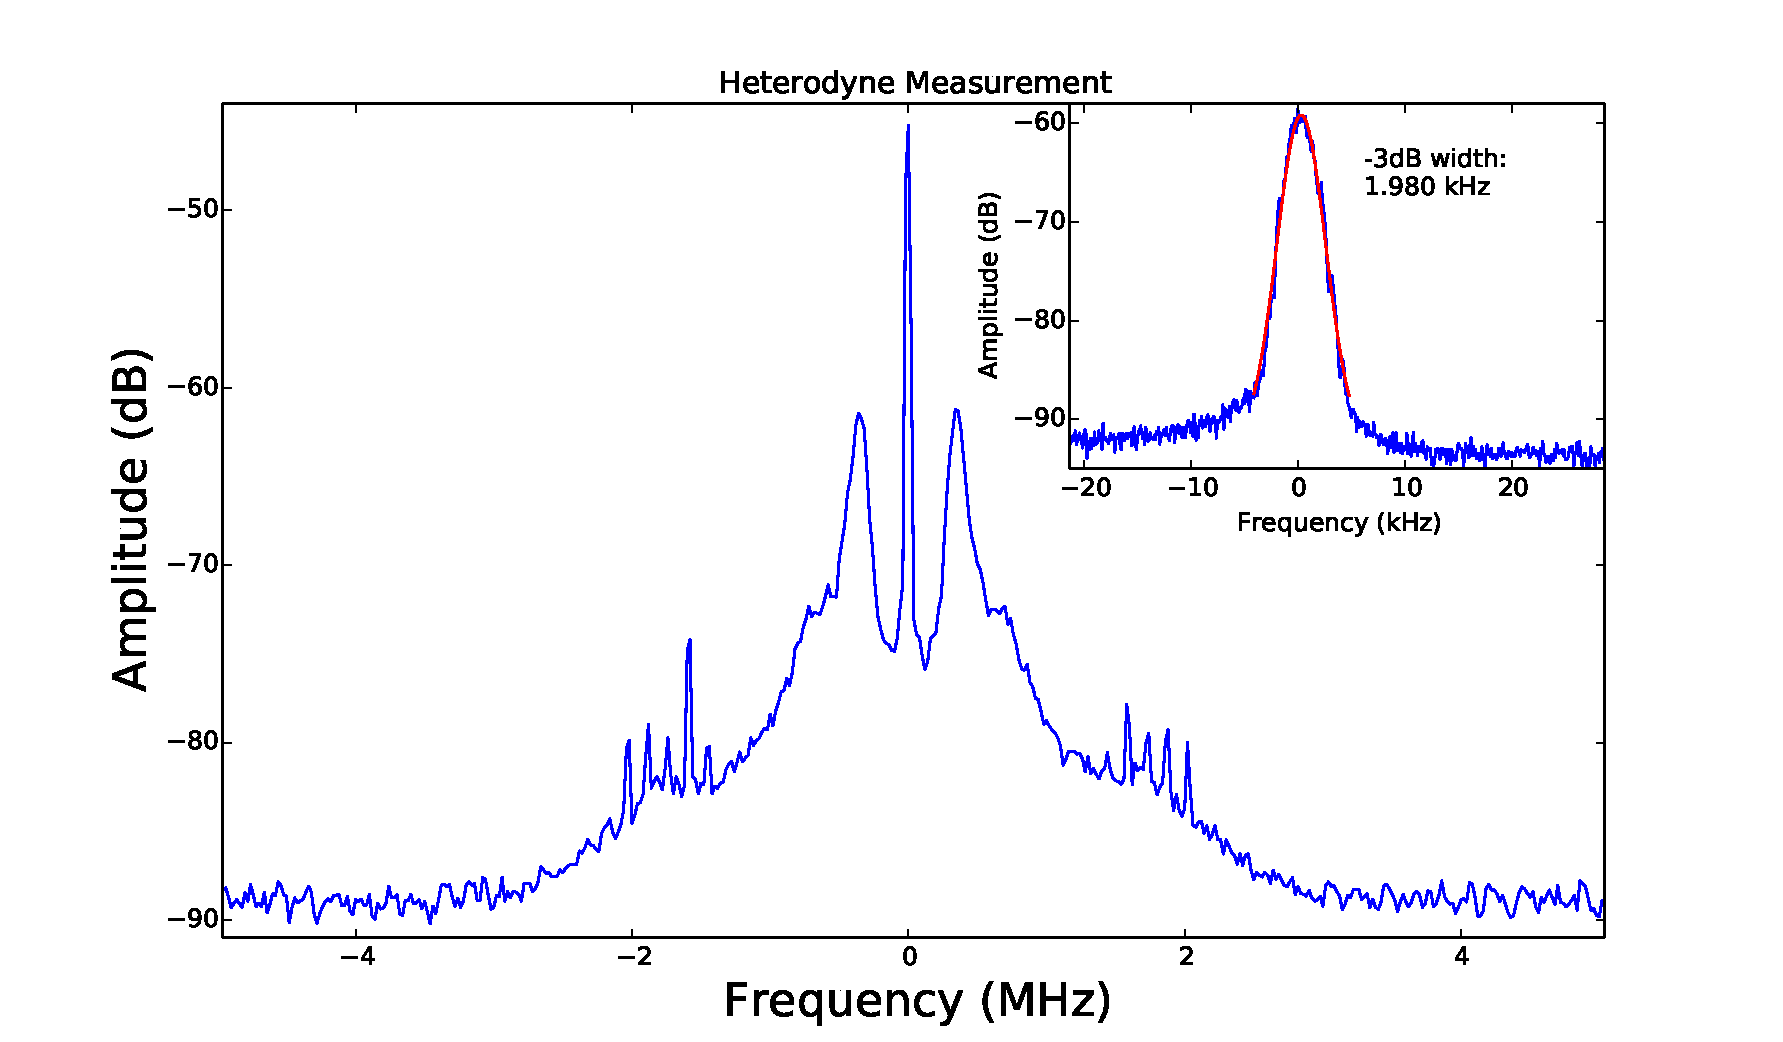
\includegraphics[width=\linewidth]{Figs/beatnote_inset.pdf}
%%    \captionsetup{type=figure}
%%    \captionof{figure}{Typical heterodyne beatnotes for the two lasers locked with \gls*{ps}. Both measurements are 50 shot averages taken consecutively. Something like this. Caption still WIP.}
%%    \label{beatnote}
%%\end{Figure}
%
%\section{Conclusion}
%
%The spectral linewidth achievable with \gls*{ps} is demonstrably lower than previously indicated. The current limiting factor is the bandwidth of the electronics used. It is likely that due to \gls*{ps} not being temporaly limited by atomic population evolution that with higher bandwidth electronics and additional work into vibrational stability that the linewidth could be further reduced. The current experimental setup is an example of a low cost, low linewidth and simple laser source frequency stabilised to an atomic reference.
%
%\section{Acknowledgements}
%\begin{itemize}
%\item Funding sources.
%\item Alex for electronics help (or should he be an author?)
%\item Rory for sanity checking of code (hrm... probably not going to be using those results in the paper after all. Remove acknowledgement?)
%\item Andre Luiten for equipment and advice
%\end{itemize}
%
%\bibliographystyle{plain}
%\bibliography{Library,Equipment}

%\end{multicols}
\end{document}
